\section*{Discussion}
\label{sec:discussion}

That \ac{NSC} can explain and reproduce response properties observed in biological neurons may be an important clue as to how brains have evolved to parse and store information
in order to perceive the world and interact with it.
We offer three testable predictions of this theory:

First, we suggest that a variety of neuronal response properties
can be understood as an emergent property of efficient population coding 
based on dimensionality reduction.
Depending on input stimulus and task complexity,
we expect the dimensionality of the population code to be adjusted
according to the bias-variance dilemma
(Fig.~\ref{fig:nsc-bias-variance-dilemma}).
This point of operation might differ across brain areas---for example,
favoring neurons that respond to a small number of stimulus dimensions
in \ac{V1} \cite{OlshausenField1996},
but giving rise to mixed selectivity in higher-order brain areas
such as \ac{MSTd} \cite{Beyeler2016},
\ac{RSC} \cite{Rounds2016,Rounds2018},
and \ac{PFC} \cite{Mante2013}.

Second, we predict that parts-based representations can explain
\acp{RF} of neurons in a variety of brain regions,
including but not limited to those brain areas discussed here. 
In agreement with the literature on basis function representations
\cite{PougetSejnowski1997,PougetSnyder2000,Poggio1990},
we expect parts-based representations
to be prevalent in regions where neurons
exhibit a range of tuning behaviors \cite{Beyeler2016},
display mixed selectivity \cite{Fusi2016,Eichenbaum2017},
or encode information in multiple reference frames \cite{AlexanderNitz2015,Rounds2016,Rounds2018}.

Third, where such representations occur, we expect the resulting
neuronal population activity to be relatively sparse,
in order to encode information both accurately and efficiently.
As noted above,
sparse codes offer a trade-off between 
dense codes (where every neuron is involved in every context,
leading to great memory capacity but suffering from cross talk among neurons)
and local codes (where there is no interference, 
but also no capacity for generalization).
\ac{NSC} explicitly discourages statistically inefficient representations,
because strongly accounting for a rare observation at the expense of ignoring
more common input components would result in an increased reconstruction error
(see Eq.~\ref{eqn:nsc-cost-function}).


\subsection*{\revise{Potential for NSC in nonsensory areas of the brain}}

\mikeNote{R1: In the previous round of reviews, I already suggested that the authors’ model seems more appropriate for sensory areas, and that it may not apply to the motor system. Despite the changes to the paper, I think the paper would be clearer and perhaps more compelling that way. To be clear, I’m not arguing that the authors should complete remove non-sensory areas, but I think it should be a part of the Discussion ``Would these ideas apply to non-sensory areas?'' rather than of the core of the paper.}
\revise{In addition to the areas highlighted above,
there is increasing evidence that the essential components of \ac{NSC}
might be present in numerous brain regions 
not traditionally associated with the efficient encoding of information.}

\revise{For example, there is evidence for sparse coding in the
cerebellum \cite{Marr1969,Schweighofer2001,Brunel2004},
\ac{PFC} \cite{Abeles1990,Fujisawa2008,Wei2015},
motor cortex \cite{Beloozerova2003,Kakei2003,BarthPoulet2012,Brecht2004},
hippocampus \cite{rolls2013,ThompsonBest1989,Poli2017,Wixted2014},
and the amygdala \cite{Bach2011}.
Similarly, there is evidence for dimensionality reduction in
\ac{PFC} \cite{Mante2013}
and motor cortex \cite{Graziano2009,Gallego2017}.
However, the intrinsically complex response properties of individual neurons
have defied a deep understanding of how these neurons contribute to behavior
\cite{churchland2007,Mante2013}.
For example, individual \ac{PFC} neurons typically encode multiple task-related signals
at once, including the animal's upcoming choice, the context,
and the strength of the sensory evidence \cite{Mante2013,Rigotti2013,Kobak2016}.
Future studies may show that key features of the population response in these regions
can be recovered by applying \ac{NSC} to their inputs.}

\revise{Analogous to our modeling work in \ac{MSTd} \cite{Beyeler2016},
it might be possible to apply \ac{NSC} to other areas of the posterior parietal
cortex that are involved in multisensory heading perception.
Areas such as the \ac{VIP} and \ac{VPS} are also known to respond to optic flow,
but they increasingly respond to inertial vestibular stimulation as well
\cite{Chen2011}.
Although the degree of sparsity of the population code in \ac{VIP} and \ac{VPS} is not known,
the fact that neurons in these areas respond to mixtures of visual and vestibular
heading cues make them prime examples 
to be examined with an \ac{NSC} based modeling approach.}

\revise{Elsewhere in parietal cortex, single neurons act as basis functions 
to represent the spatial configuration of objects 
with respect to multiple reference frames
(e.g., by transforming eye-centered to body-centered coordinates).
\cite{Poggio1990,PougetSejnowski1997,PougetSnyder2000}.
This is similar to the integration of multimodal heading cues mentioned above,
as well as to other associative areas such as \ac{RSC},
which demonstrates conjunctive coding of various spatial navigation cues
\cite{AlexanderNitz2015,Rounds2018}.
There is further evidence that actions are represented in parietal cortex
with respect to arbitrary and abstract reference frames, 
such as with respect to a planned route through an environment \cite{nitz2009parietal}.
From a theoretical standpoint, \ac{NSC} seems a good candidate to find an efficient,
reference-frame agnostic representation of various behaviorally relevant variables
\cite{LouieGlimcher2012,louie2015adaptive,andersen1997multimodal,BenHamed2003},
but future studies will have to address these issues step by step.}



\subsection*{Potential neural mechanisms of NSC}

As a special case of efficient coding,
\ac{NSC} possesses metabolic advantages by employing
sparse population codes.
To operate efficiently, it has been suggested that the brain might enforce 
geometrical and biophysical constraints on axonal wiring 
\cite{LaughlinSejnowski2003}.
In addition to reducing overall wiring length
\cite{Cherniak1994}, the brain might also aim to minimize local delays
by favoring a high degree of local connectivity
\cite{Chklovskii2002}.
\revise{If connectivity reflects} coding \cite{Clopath2010},
it would not be surprising to find that such ecological considerations
carry over into brain function,
favoring sparse population codes and neuronal representations that are
local in functional space (i.e., parts-based).
However, wiring cost is likely to be only one of many constraints 
on the brain connectome, perhaps supplementing competitive pressures
for hub-mediated information exchange between network modules
\cite{Rubinov2015}.

In addition, evidence suggests that Hebbian-like synaptic plasticity rules
allow neurons to perform statistical inference on their inputs
\cite{Nessler2009,Carlson2013,MorenoBoteDrugowitsch2015,Oja1982}.
One particular study demonstrated through a mathematical proof
that a certain form of \textbf{\ac{STDP}} in combination with 
homeostatic synaptic scaling (i.e., \ac{STDPH})
can approximate the \ac{NMF} algorithm
\cite{Carlson2013}.
Similar to Oja's rule \cite{Oja1982}, which was developed to stabilize 
rate-based Hebbian learning
(effectively resulting in principal component analysis),
Carlson and colleagues showed that synaptic scaling acts as a 
homeostatic mechanism to stabilize \ac{STDP}
(effectively resulting in \ac{NMF}).
Interestingly, we were able to apply these ideas to 
electrophysiologically recorded neuronal activity observed in the \ac{RSC}
of rats during a spatial navigation task (Fig.~\ref{fig:NMF|RSC}; for experimental details see Supplementary Material). Both \ac{STDPH} and \ac{NMF} were able to recover key  features such as encoding spatial reference frames (i.e., allocentric and route-centric firing patterns) and position discrimination by reducing the dimensionality of behavioral variables (e.g., velocity, head direction, position).
The neuronal and population responses from NMF and STDPH were comparable to the experimental findings \cite{AlexanderNitz2015}.
Furthermore, the \ac{STDPH} model contained a highly flexible and generalizable code
that could automatically encode new routes through the same environment
without retraining \cite{Rounds2018}.
However, more research is needed to elucidate any potential connection 
between \ac{NSC} and the many different synaptic plasticity rules 
commonly found across brain regions,
different stages in the life of an animal, and animal species
(e.g., \cite{Froemke2010,BCM1982}).
\mikeNote{R1:  Fig 8 is hard to interpret, what is the percent model error? Does this error reflect a ``movement prediction error''?}

\begin{figure}[h]
	\centering
	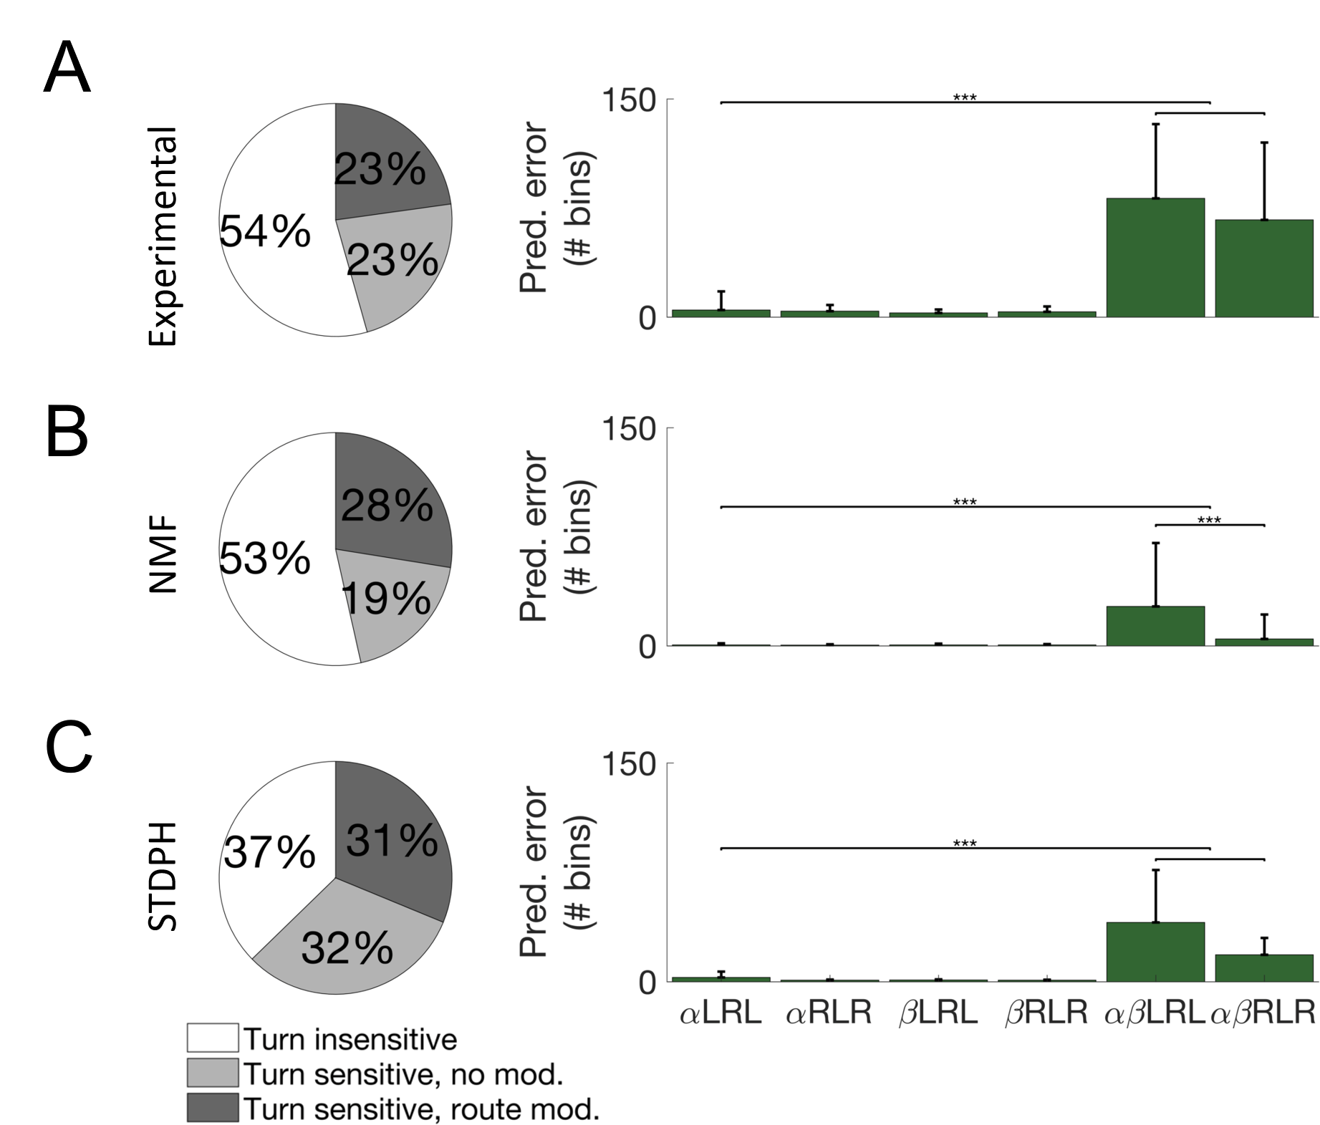
\includegraphics[width=\textwidth]{fig-rev1-rsc}
    \caption{
    	Comparisons between recorded experimental data and two 
        computational models of rat \ac{RSC} suggest a functional 
        similarity between \ac{STDPH} and \ac{NMF} 
        (adapted from \cite{Rounds2018}). 
        Using methods described in \cite{AlexanderNitz2015}, 
        we compared functional neuron type distributions (left column)
        and average prediction errors (right column)
        observed \emph{in vitro} (\textbf{\emph{A}}) with those
        produced by each model (\textbf{\emph{B, C}}).
        Average error corresponded to correlation matrices 
        representing reconstructed position within a route. 
        For details, see Supplementary Materials.
        Separate positions of the W-shaped track are represented 
        by the symbols $\alpha$ and $\beta$. 
        Outbound and inbound runs were made up of 
        opposite turn sequences (left-right-left (LRL) 
        and right-left-right (RLR), respectively.
        Reconstructions between the track positions are represented by
        $\alpha \beta$.
	    \textbf{\emph{A}},
    		Experimental data from \cite{AlexanderNitz2015}.
        \textbf{\emph{B}},
            Simulated using NMF with sparsity constraints.
        \textbf{\emph{C}},
            Simulated by evolving \ac{STDPH} parameters 
            to fit experimental data \cite{BeyelerCarlsonChou2015,Carlson2014}.
    }
	\label{fig:NMF|RSC}
\end{figure} 


\subsection*{Model limitations}

Although \ac{NSC} has proved useful in understanding
a variety of neuronal responses
as an emergent property of efficient population
coding based on dimensionality reduction and sparse coding,
there are some limitations to this theory.
\mikeNote{R1: I think the authors should mention the emerging idea that sensory areas carry a lot of information about the behavior, even visual areas [10, 12]. This information may make the activity of a sensory neuron not be just an efficient code of the stimulus.}

First, it remains to be demonstrated whether \ac{NSC} in its current form
can be extended to brain areas that require a dynamic process of information
gating, such as \ac{PFC} \cite{Mante2013,Rigotti2013,Kobak2016}
and motor cortex \cite{Vargas2010decoding,GrazianoAflalo2007}.
In these areas, diverse time courses across neurons have confounded
attempts to understand the basic encoding of decisions and movements.
\mikeNote{R1: when the authors mention the different time courses of neural activity across areas, maybe they want to mention that in motor areas activity seems to be well-represented by RNNs, whereas in visual areas feedforward nets seem to be better models?}
However, the same is true for the olfactory system,
where population activity traces out loops that are organized by stimulus
condition. In particular, the orientation of the loop 
is related to the odor identity,
and the size of the loop is related to the odor concentration
\cite{Broome2006}.
Nevertheless, a recent \ac{NSC} based study was able to elucidate perceptually
relevant dimensions in odor space \cite{Castro2013}.
Our hope is that similar studies applied to \ac{PFC} and motor cortex will
reveal similar insights into their population response properties.

Second, a practical limitation of dimensionality analyses in general
is that the apparent dimensionality of the population response changes
systematically with the complexity of the input stimulus
\cite{SpanneJorntell2015,Cowley2016,Mazzucato2016}.
For practical purposes, simulated models of neuronal circuitry are typically
built with far fewer units than the number of neurons in the real network.
By excluding input dimensions that are present in the brain,
one will implicitly guide the simulated model away from spurious interactions
that the real circuitry would have to handle.
As a result, the simulated model might underestimate 
the true complexity of the task.

Third, the role of sparse coding in the brain has been questioned
\cite{SpanneJorntell2015,BarthPoulet2012}.
This is at least partly due to the wide variety of definitions of sparse
coding used in the literature:
In its widest possible theoretical sense,
a neuron population exhibits sparse activity if the average activation ratio
remains below 50\% for binary neurons 
or below 100\% for thresholded,
rate-based neurons \cite{SpanneJorntell2015}.
However, it is not surprising that different brain areas might employ
different degrees of sparsity.
\mikeNote{R1: These paragraphs are not very clear, starting with the authors’ definition of learning... Please rewrite}
Whereas learning can be extremely fast in a local code,
a network of `grandmother' cells suffers from low representational capacity.
As the degree of sparsity in the network decreases and the code gets denser,
representational capacity and fault tolerance 
(i.e., the capacity to handle neuronal noise or the loss of a subset of neurons)
improve,
but at the expense of a decrease in learning speed
\cite{Foldiak1990,SpanneJorntell2015}.
The optimal point of operation would therefore depend on the complexity of
the stimulus to be encoded or the task to be performed,
subject to constraints on the required speed of learning.
This point of operation might differ drastically across brain areas---for example,
favoring an extremely sparse code in \ac{V1}
\cite{OlshausenField1996},
but giving rise to a slightly denser code with 
greater representational capacity in higher-order visual areas
such as \ac{MSTd}, 
which could lead to compact and multifaceted encodings
of various perceptual variables
(see Discussion in \cite{Beyeler2016}).


\subsection*{Model alternatives}

Since \ac{NMF} is an integral part 
of Eq.~\ref{eqn:nsc-cost-function},
it is interesting to note that \ac{NSC} is tightly connected
to a number of unsupervised learning techniques,
such as $k$-means clustering,
an algorithm used to partition
$n$ observations into $k$ clusters
\cite{Ding2005}.
Due to its ability to decompose high-dimensional data into
sparse, interpretable factors, \ac{NMF} has become a 
widely used tool for the analysis of high-dimensional data,
with applications reaching far beyond
the field of computational biology
(for a recent review see \cite{Gillis2014}).

In addition to the tight connection 
to linear sparse coding and \ac{NMF}
\cite{EggertKorner2004},
\ac{NSC} is also intimately related to \textbf{\ac{ICA}},
a computational method for separating a multivariate signal
into additive, statistically independent subcomponents. 
As originally noted by Hoyer \cite{Hoyer2002},
if the fixed-norm constraint is placed on the rows of
\textbf{H} instead of the columns of \textbf{W},
Eq.~\ref{eqn:nsc-cost-function} can be directly interpreted as the joint
log-posterior of the basis functions and hidden components
in the noisy \ac{ICA} model \cite{HoyerHyvarinen2002}.
In order for this connection to hold,
the \ac{ICA} basis functions must be chosen to be nonnegative,
and the independent components must have 
exponential distributions \cite{Hoyer2002}.

Similarly, \ac{NSC} is closely related to compressed sensing
(for a recent review see \cite{GanguliSompolinsky2012}),
and a recent study has even suggested to combine the two
\cite{WangLi2010}.
Compressed sensing posits that neurons might implement 
\mikeNote{R1: recent paper from the Shenoy and Ganguli labs [13] that shows that this notion applies to M1 data}
dimensionality reduction by randomly projecting patterns of activity
into a lower-dimensional space,
simply by synaptically mapping $N$ upstream neurons to a downstream region
containing $M < N$ neurons.
The theory of compressed sensing then provides the mathematical tools
to reconstruct the original space from the random projections.
\ac{NSC}, \ac{ICA}, and compressed sensing often make similar predictions
that only slightly differ in the nature of the basis function representation
necessary to achieve optimal reconstruction
(for details please refer to the Discussion of \cite{GanguliSompolinsky2012}).
For example, whereas \ac{ICA} emphasizes the statistical independence 
of unmixed sources
and compressed sensing requires basis function to be `maximally incoherent'
\cite{GanguliSompolinsky2012},
\ac{NSC} does not make any such assumptions
as long as the basis functions are nonnegative.
